\chapter{Revisão Bibliográfica} \label{chap:sota}


\section{Definição e caraterização do problema}\label{sec:problem}

Com a modernização constante da indústria e consequente crescente exigência
de conetividade de todo o tipo de equipamentos, é imperativa a introdução
de novas soluções tecnológicas que satisfaçam estes requisitos modernos
mas que também mantenham a compatibilidade com as exigências satisfeitas
pelos sistemas atualmente em uso.

Quando nos referimos à área da robótica, exigências temporais como o
período, a latência e a periodicidade da malha de controlo são fulcrais
para o funcionamento estável do sistema. Ora, a crescente exigência de
conetividade moderna instiga à utilização de redes de comunicação no
ambiente industrial. Quando o controlo de diversas áreas num equipamento
é feito de modo central num PLC ou micro-controlador, a sincronização de
alteração de estados de saídas é trivial, pois basta garantir que ambas
são atualizadas no mesmo ciclo de processamento. Quando se pretende
introduzir uma rede de comunicação entre o processamento central e o
controlo das saídas e/ou a aquisição das entradas, é crucial garantir
que não existem atrasos significativos na transmissão da informação
na rede e garantir a sincronização entre as atualizações das saídas
nos diversos escravos.

Nos últimos anos, várias implementações e estudos já foram realizados
com manipuladores robóticos utilizando redes de comunicação na malha de
controlo como \cite{Zhang18}, \cite{leiwang2010} ou muito recentemente
\cite{deremetz2020}. No entanto, todas elas se focam na vertente mais
industrial e técnica da solução e praticamente não existem implementações
focadas no ensino.

% económico
Um demonstrador focado no ensino deve ter caraterísticas apelativas de
modo a que a sua utilização possa ser o mais generalizada possível. O
primeiro objetivo deverá ser o desenvolvimento de um produto de baixo
custo, de forma a que este possa ser adquirido em larga escala pelos
estabelecimentos de ensino. É também preciso considerar que no ambiente
de ensino, é mais provável o acontecimento de situações de utilização
indevida de um equipamento comparativamente a um ambiente industrial,
onde geralmente apenas pessoal qualificado está autorizado a interagir
com este, e portanto uma possível avaria do mesmo não pode trazer
prejuízos avultados à instituição e/ou ao estudante. Naturalmente, esta
redução no custo implicará sempre uma redução na qualidade do produto
final face a um desenvolvimento de nível industrial, mas essa não é uma
caraterística fundamental de um demonstrador didático, pois o seu principal
objetivo é a transmissão e/ou auxílio na compreensão do conhecimento.

% implementação simples
Tipicamente no momento em que nos é apresentada uma tecnologia desconhecida
através de um demostrador didático surgem questões acerca do demostrador
propriamente dito e não na tecnologia que ele pretende demonstrar. É,
portanto, necessário desenvolver equipamentos focados no ensino que não
imponham este tipo de barreira ao processo de aprendizagem. Assim,
para minimizar este tipo de interferências existem duas possíveis soluções:
utilizar um conceito que seja tão simples quanto possível, de modo a
não permitir qualquer tipo de dúvida; ou que o público alvo tenha um
conhecimento aprofundado do conceito de base do demonstrador. Considerando
que este demostrador será direcionado a estudantes de mestrado na área da
robótica, o controlo de movimento e posição é um tema bem conhecido.

% componentes 'off the shelf'
Complementando a caraterística económica de um demonstrador educativo,
a utilização de componentes e sub-sistemas genéricos, denominados
componentes \emph{off-the-shelf}, facilita a aquisição dos mesmos tanto
para efeitos de fabrico como para efeitos de reparação. Assim, é possível
que o próprio cliente faça uma reparação do produto, sendo que a solução
mais simples e prática será a troca do componente ou sub-sistema danificado.

% modularidade
A utilização de componentes e sub-sistemas genéricos leva-nos a mais uma
caraterística importante de demonstradores educativos: a modularidade. Um
sistema dividido em secções simples que se focam numa única tarefa é um
sistema modular. Em engenharia dá-se o nome de sub-sistema a cada uma
dessas secções. Cada sub-sistema por si é simples, fácil de implementar,
interpretar e diagnosticar. A inter-ligação dos diferentes sub-sistemas
permite obter um sistema mais complexo e o seu desenvolvimento e eventual
diagnóstico pode ser feito por partes, simplificando o processo, e
proporcionando também a possibilidade de este ser paralelizado.
Esta modularidade permite que, no contexto de aprendizagem, seja mais
fácil e rápido interpretar o funcionamento de cada sub-sistema e,
consequentemente, o funcionamento geral do sistema.

% reprodutibilidade
A agregação das últimas três caraterísticas (simplicidade, modularidade
e utilização de componentes genéricos) origina mais uma caraterística
importante de um demonstrador didático: a reprodutibilidade. Para muitas
instituições de ensino é importante que este tipo de equipamentos seja
facilmente reprodutível, pois muitas preferem produzir os seus próprios
equipamentos, escolhendo os componentes a usar. Isto permite a cada
instituição gerir a quantidade de equipamentos existentes e, inclusivamente,
proporciona a possibilidade de efetuar reparações no local. O próprio ato
de montagem de um equipamento educativo é interessante para auxiliar o
lecionamento do tema abordado.

% intuitivo
Por fim, uma das caraterísticas mais importantes de qualquer demonstrador
educativo, e razão pela qual estes existem, é o seu caráter intuitivo.
Qualquer utilizador deve ser capaz de, através do próprio funcionamento
do demonstrador, entender o conceito base em exposição. Em ambiente
educacional é muito importante fornecer este tipo de contacto com a
tecnologia para que os estudantes possam sedimentar os conhecimentos com
mais facilidade e de uma forma mais duradoura. % TODO arranjar citação para isto


\section{\ecat}\label{sec:ethercat}

A rede \ecat\ é uma rede de \emph{Ethernet} industrial que usa a
especificação padrão IEEE 802.3 \cite[]{ieee:IEEEStandardEthernet} para
definir o formato dos \emph{frames} e camada física a utilizar, mas
introduz uma maneira diferente de os processar.

Esta nova forma de processamento permite uma comunicação com todos os
dispositivos presentes na rede com apenas um \emph{frame}. \ecat\ utiliza
uma tipologia de comunicação \emph{Master/Slave}, tipicamente implementada
numa arquitetura de rede encadeada (\emph{daisy-chain}), mas permite várias
outras arquiteturas.

\subsection{Princípio de funcionamento}

A rede \ecat\ utiliza como base um \framee\ \ethernet\ padrão, fazendo
uso do endereçamento MAC e inserindo os seus datagramas de comunicação no
conteúdo do \framee\ \ethernet. Estes são marcados com o identificador
0x88A4 no campo \emph{Ethertype}. Isto permite que as comunicações \ecat\
não dependam da pilha de protocolos de comunicação tradicionais como
\emph{TCP/IP} ou \emph{UDP/IP}. A figura \ref{fig:ecat-frame}, retirada
da página de apresentação da tecnologia \cite[]{group:EtherCAT}, demonstra
o aspeto genérico da estrutura de um \framee\ \ecat.

\begin{figure}[htp]
 \centering
 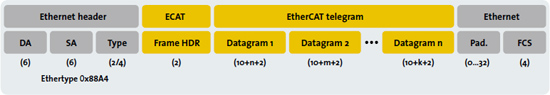
\includegraphics[width=\linewidth]{EtherCAT_Technology_01_Protocol.jpg}
 \caption{Estrutura de um \emph{frame} \ecat}
 \label{fig:ecat-frame}
\end{figure}

Vários datagramas de \ecat\ podem ser transmitidos no mesmo \framee\ \ethernet\
de modo a otimizar a eficiencia da transferência de informação. Durante
a configuração da rede, o dispositivo mestre atribui um ou mais endereços 
a cada escravo, de maneira que é possível endereçar cada escravo individualmente
ou endereçar grupos de escravos em simultâneo. Este processo é denominado
endereçamento lógico e permite separar os dados relativos a diferentes
tarefas geridas pelo dispositivo mestre. Cada datagrama enviado no
\framee\ \ethernet\ terá um cabeçalho que indicará qual o tipo de acesso
que o dispositivo mestre pretende efetuar com o(s) escravo(s) identificado(s)
no datagrama. Os acessos disponíveis são apenas leitura, apenas escrita
ou leitura e escrita em simultâneo.

Apenas o dispositivo mestre pode iniciar um \emph{frame} de comunicação
e os dispositivos escravos limitam-se a ler a parte informação contida
no \emph{frame} que lhes é endereçada. Ao mesmo tempo, cada dispositivo
escravo pode introduzir informação sua  no \emph{frame} antes de o enviar
para o dispositivo seguinte.

Através destas funcionalidades de endereçamento lógico e da definição do
modo de acesso em cada datagrama, o dispositivo mestre pode decidir quando
pretende ler ou escrever dados de cada escravo, permitindo assim que se
configurem diferentes períodos de atualização para cada tarefa, como por
exemplo, fazer uma atualização dos parametros dos controladores dos motores
com período de 1ms e fazer a atualização dos comandos manuais do utilizador
com período de 10ms.

\subsection{Arquiteturas de rede}
\label{sec:daisychain}
Como referido em \ref{sec:ethercat}, esta rede é muito flexível em termos
da topologia de rede que suporta. As mais comummente utilizadas são
a encadeada, em árvore ou em estrela e é possível fazer uma combinação de
topologias diferentes em diversas secções da rede. A imagem 
\ref{fig:ecat-topology}, retirada da página de apresentação
\cite[]{group:EtherCAT}, demonstra estas topologias numa configuração mista.

\begin{figure}[htp]
 \centering
 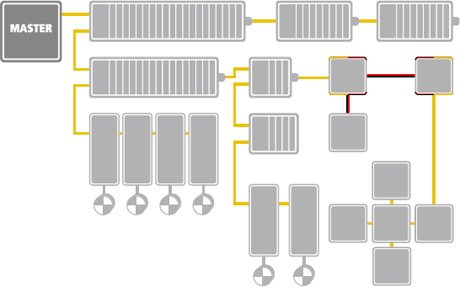
\includegraphics[width=\linewidth]{EtherCAT_Technology_03_Topology.jpg}
 \caption{Configuração mista de topologias suportadas pela rede \ecat}
 \label{fig:ecat-topology}
\end{figure}


\subsection{Sincronização de relógios}
Em aplicações onde é necessário garantir a simultaneidade de ações, como
discutido em \ref{sec:problem}, a utilização de uma arquitetura distribuída
com base em redes de comunicação dificulta o processo de manter o bom
funcionamento de ações síncronas. Um bom exemplo é, exatamente, um sistema
que envolve a sincronização de movimentos multi-eixo.

A rede \ecat\ colmata esta dificuldade através da utilização de um sistema
de sincronização de relógios distribuídos (\emph{distributed synchronised
clocks}). A calibração dos relógios é implementada na íntegra no
\emph{hardware}, fazendo a distribuição cíclica do valor do relógio do
primeiro dispositivo escravo por toda a rede, resultando numa sincronização
dos relógios de todos os dispositivos escravo com um valor de \emph{jitter}
abaixo de 1 microssegundo. Este valor significa que o relógio a que ele
diz respeito têm um desvio relativamente ao relógio de referência de,
no máximo, 1 microssegundo. Durante o período de inicialização da rede,
esta operação de sincronização de relógios mede o tempo de transmissão
dos dados no meio de transporte e aplica a devida compensação.

Quando todos os dispositivos têm os relógios sincronizados, estes podem
atualizar as saídas no mesmo instante e fornecer um registo temporal
muito preciso da aquisição das entradas. Como já foi apresentado em
\ref{sec:problem}, esta funcionalidade é fundamental para o funcionamento
de sistema robóticos que façam uso de redes de comunicação nas suas
malhas de controlo. Mais à frente, quando se fizer a apresentação das
soluções propostas para esta dissertação na secção \ref{sec:solution},
ir-se-á dar exemplos concretos desta necessidade com base no conceito
de cada um dos sistemas de demonstração.


\subsection{Conclusão}
Estas caraterísticas permitem que o dispositivo mestre seja implementado
em qualquer tipo de dispositivo que contenha uma porta de comunicação 
\emph{Ethernet}. Os dispositivos escravo utilizam um \emph{EtherCAT Slave
Controller} (ESC) que processa os \emph{frames}, fazendo com que a velocidade
e tempos de resposta da rede sejam previsíveis e independentes do hardware 
em que os dispositivos escravo se baseiam. Assim, é possível a utilização
de dispositivos escravo implementados em arquiteturas de computação
diferentes dentro da mesma rede \ecat, mantendo as caraterísticas e o
desempenho da rede previsíveis.


\section{Soluções propostas} \label{sec:solution}

Para atingir os objetivos propostos por esta dissertação, foram propostas 
duas possíveis soluções. Ambas são apresentadas de seguida sendo que
maior ênfase será dada na primeira, pois é a proposta que se mostra mais
adequada ao estudo em questão. A segunda proposta é mais avançada mas
terá um custo bastante mais elevado. Como ela também depende de um manipulador
do tipo braço robótico, a sua reprodutibilidade é bastante inferior.

Ambas as soluções têm por base o controlo de movimento através da velocidade
e/ou posição de um sistema robótico de múltiplos eixos. Fazendo uso de
uma arquitetura de controlo distribuída, interligada por uma rede \ecat\
em tipologia encadeada (ver secção \ref{sec:daisychain}). Esta arquitetura
será constituída por um dispositivo mestre implementado num micro-computador
\raspi\, programado através das linguagens descritas no padrão
IEC 61161-3. Os dispositivos escravo, que farão a interface com os atuadores,
sensores e interface de comando, serão implementados através de placas
\arduino\ agrupadas com adaptadores \emph{EasyCAT} da \cite{ABT:EasyCAT}.
Um esquema simplificado da arquitetura proposta é mostrado na figura
\ref{fig:network-architecture}.

\begin{figure}[htb]
 \centering
 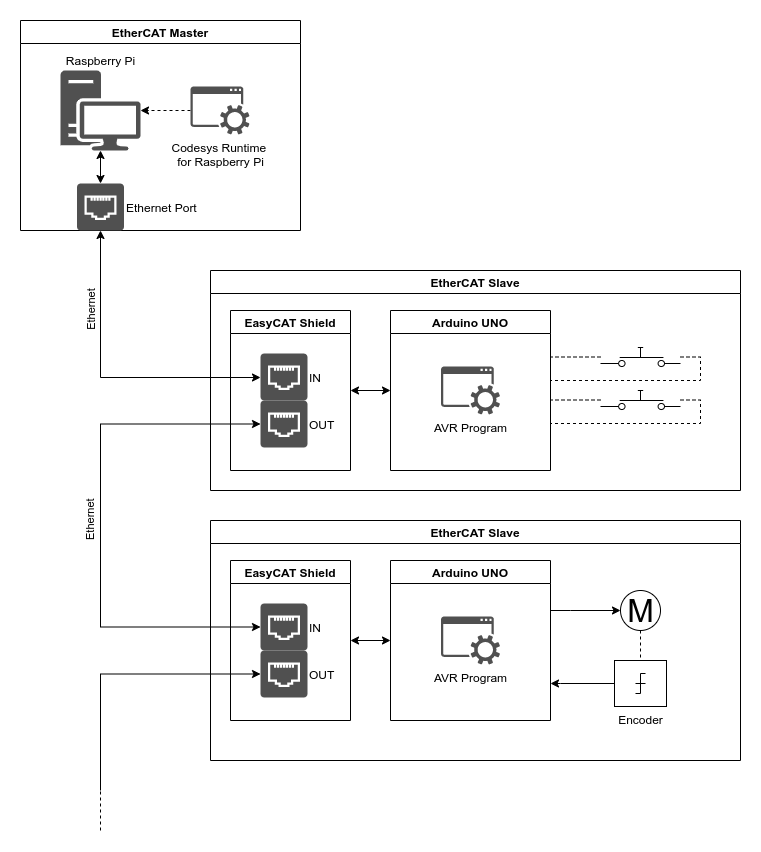
\includegraphics[width=0.8\linewidth]{network-diagram_transparent.png}
 \caption{Arquitetura da rede \ecat\ pretendida}
 \label{fig:network-architecture}
\end{figure}


\subsection{Controlo de discos perfurados}\label{sec:discs_project}

%\subsubsection{O conceito}
A primeira solução idealizada no contexto desta dissertação baseia-se num
sistema de controlo e sincronização de discos rotativos independentes.
Estes são perfurados na extremidade de maneira a que possam ser momentaneamente atravessados por um feixe de laser. Este último será fixo numa das extremidades
do demonstrador com orientação que permita atravessar todos os discos presentes
no sistema, ficando visível na extremidade oposta do demonstrador. Assim,
com estes discos acoplados a motores DC com codificadores de posição (\emph{encoder}),
controlados de forma independente por placas \arduino\ a funcionar em modo
de \ecat\ \emph{slave}, é possível criar diferentes cenários de controlo
cujo objetivo seja periodicamente alinhar as furações dos discos com o
feixe laser, permitindo que este seja viaje até à extremidade oposta.

Para complementar este conceito, será necessário permitir que o estado
do ponteiro laser (ligado ou desligado) seja controlado pelo sistema,
criando uma camada adicional de complexidade que ajuda a entender a
importância da sincronização de relógios nas redes de comunicação de
tempo real. Desta forma é possível ativar o ponteiro laser apenas quando
o sistema  determinar que os discos estão na orientação correta, fazendo
com seja mais percetível a importância da sincronização de relógios para
que seja possível uma atualização síncrona do estado das saídas.

%\subsubsection{Flexibilidade}
Idealmente esta soluçao deverá permitir efetuar o mesmo controlo mas não
usando as capacidades da rede \ecat\ e usando apenas comunicação
\emph{Ethernet} simples, o que permitirá efetuar uma comparação efetiva
destes protocolos e demonstrar que em ambientes de rede de comunicação
tradicionais não existem considerações de tempo real nem de sincronização.
Esta funcionalidade implicará verificar se os adaptadores \emph{EasyCAT}
permitem comunicação \emph{Ethernet} simples ou até de outros protocolos
de \emph{Ethernet} industrial (p.ex. \emph{Modbus TCP}), mas até ao momento
ainda não o foi possível determinar.

De forma a proporcionar um melhor entendimento sobre o funcionamento do
demonstrador aqui proposto, foi realizada uma simples simulação 3D, em
computador. Desta resultaram três imagens de pré-visualização para os
três possíveis estados do demonstrador, uma onde as furações dos discos
se alinham e o feixe de laser é visível na extremidade oposta, na figura
\ref{fig:discs1}, e duas onde as furações não se encontram alinhadas,
fazendo com que o feixe seja interrompido por um dos discos, nas figuras
\ref{fig:discs2} e \ref{fig:discs3}.

%\subsubsection{Conclusão}
Desta forma evidenciam-se as capacidades da rede \ecat\ no que diz
respeito à resposta temporal, sincronização de relógios e capacidade de
transferência de dados num sistema cujo conceito é acessível a qualquer
estudante de engenharia eletrotécnica.

\begin{figure}[htp]
 \centering
 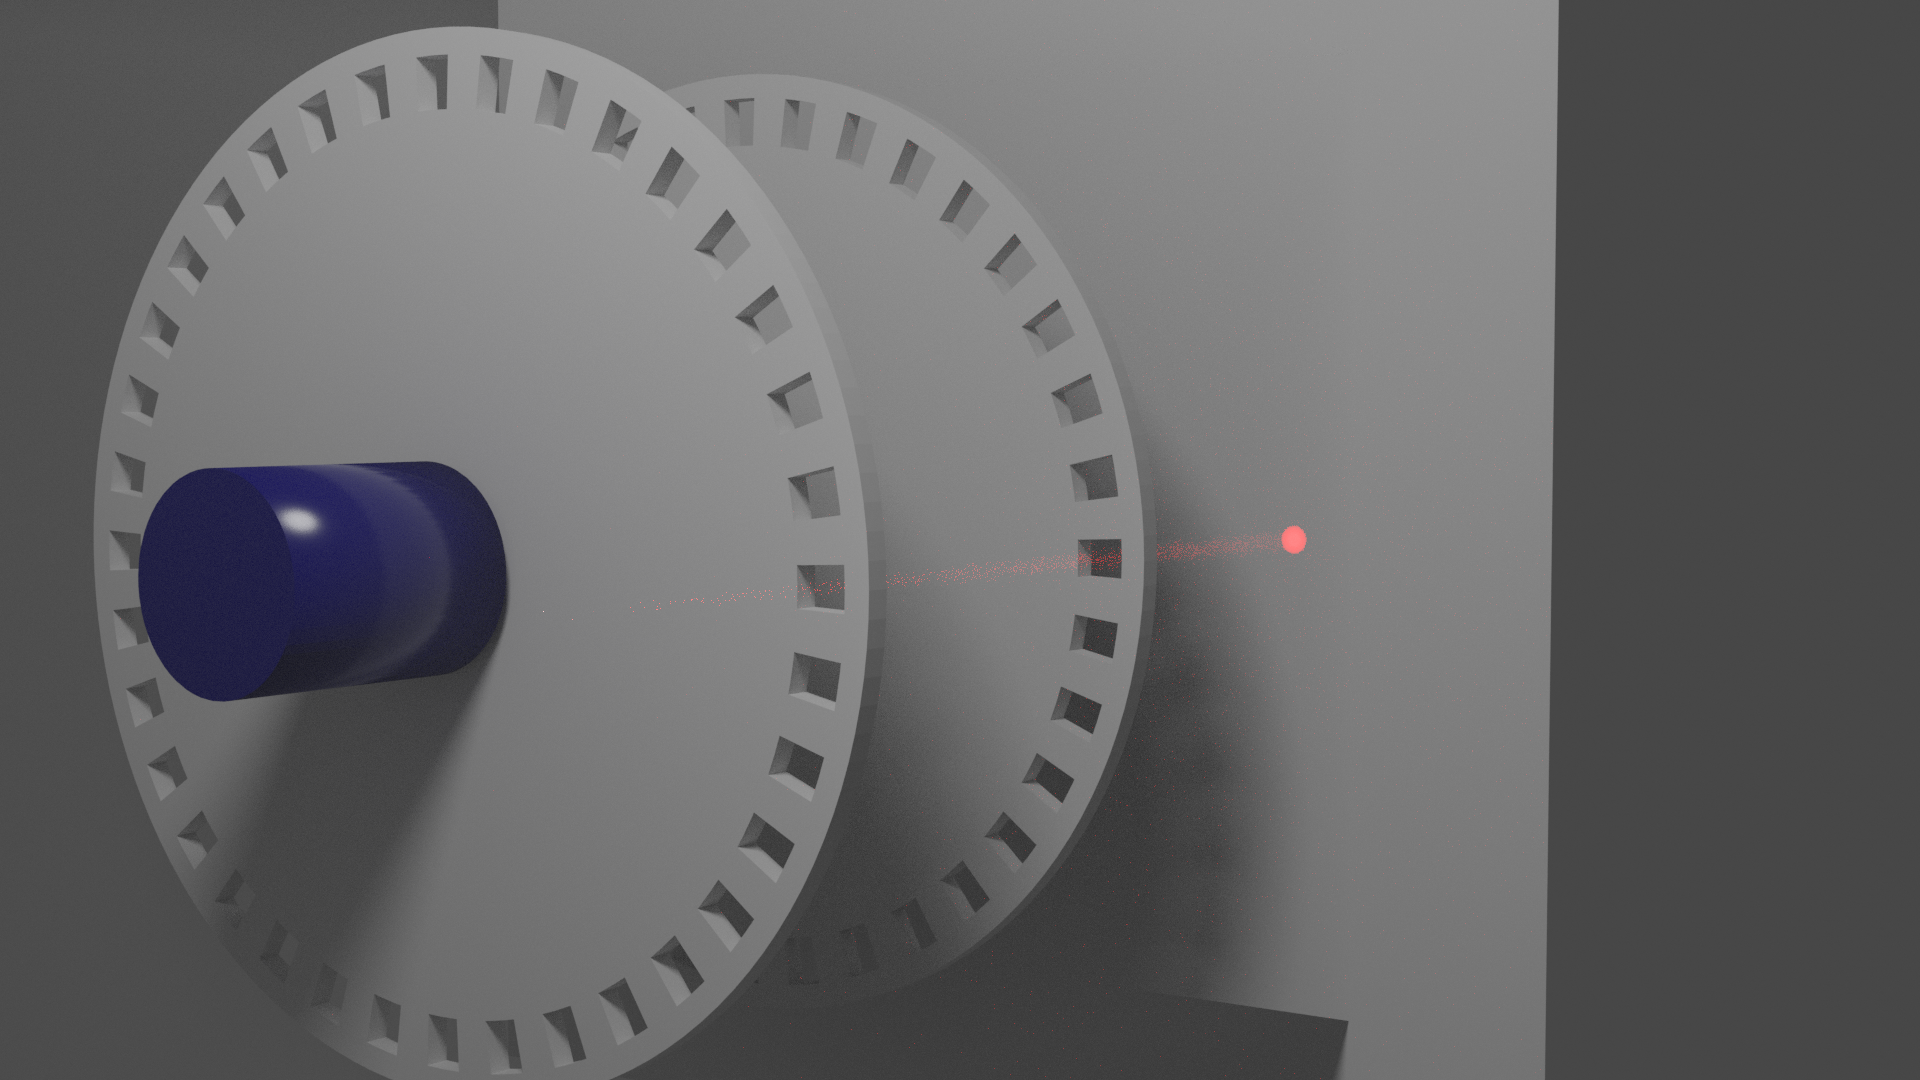
\includegraphics[width=\linewidth]{disc_1.png}
 \caption{Simulação do demonstrador - Posição 1}
 \label{fig:discs1}
\end{figure}

\begin{figure}[htp]
 \centering
 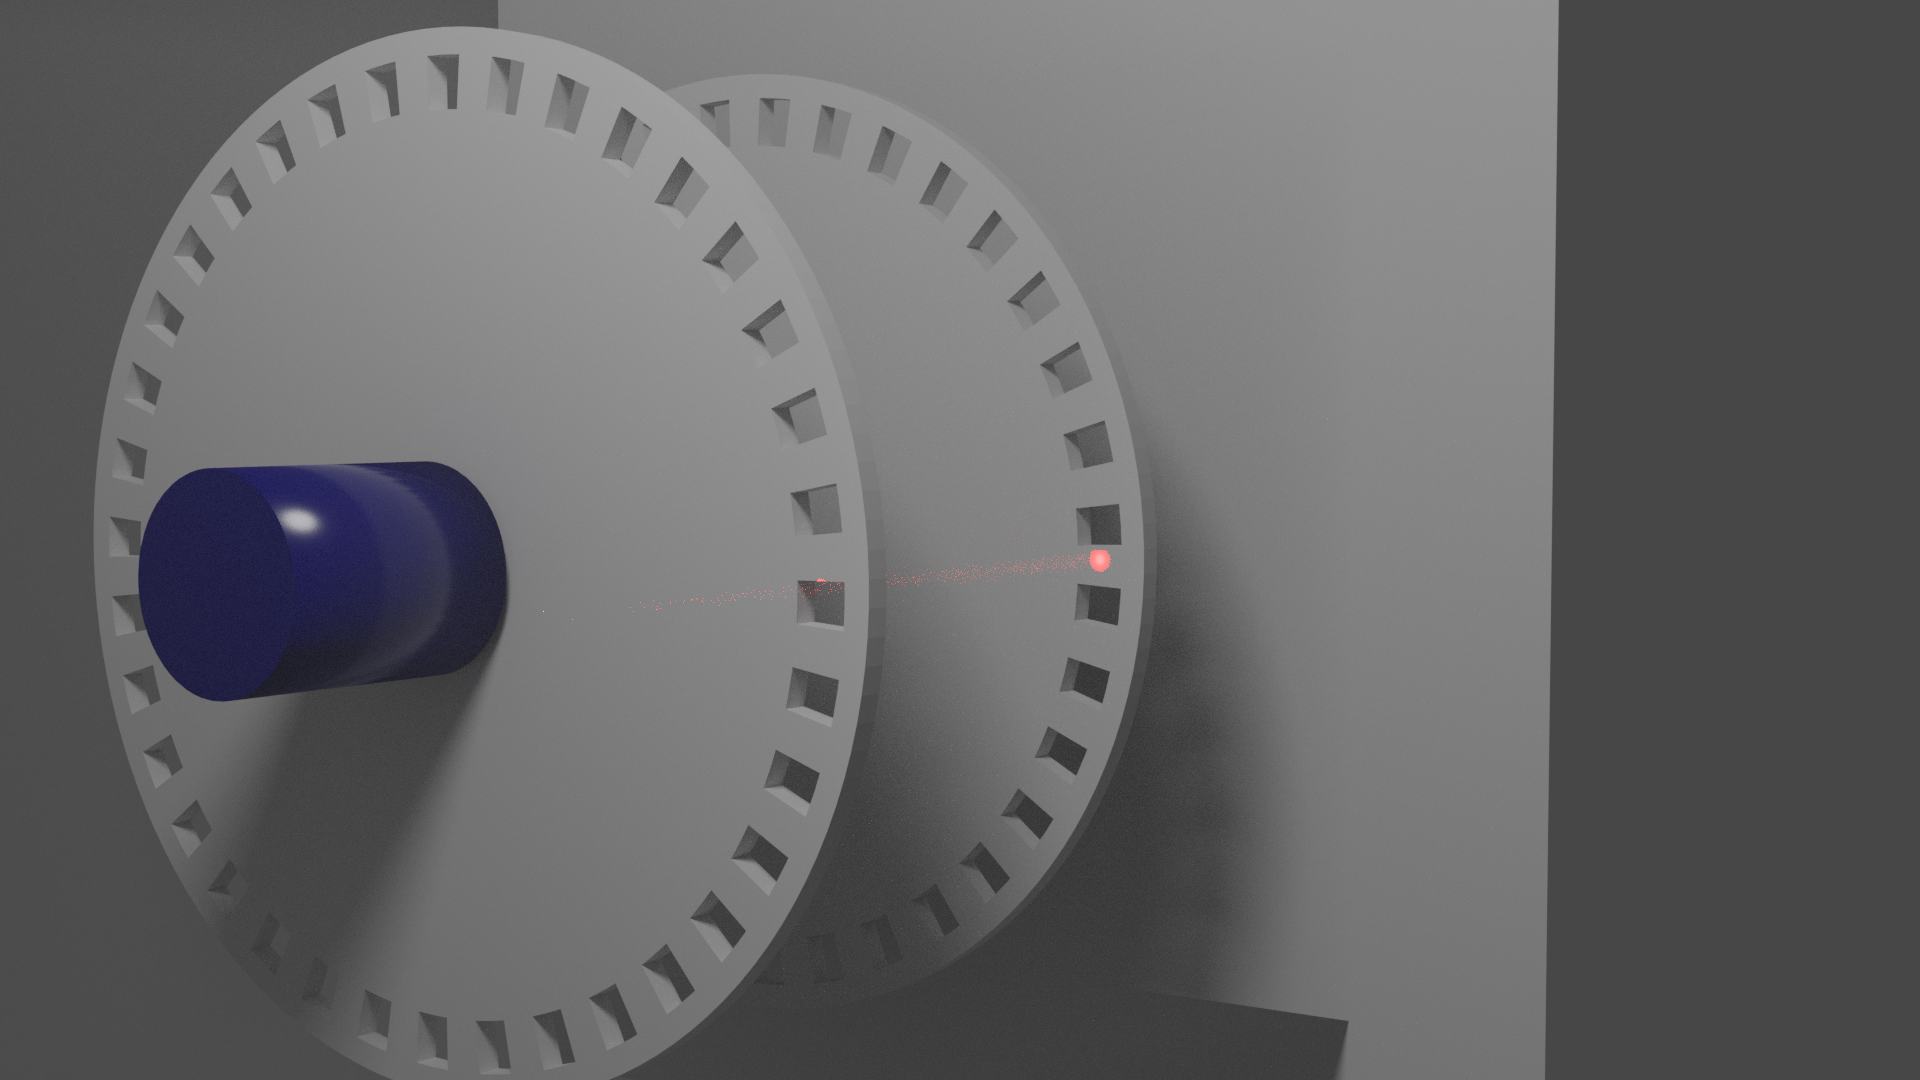
\includegraphics[width=\linewidth]{disc_2.png}
 \caption{Simulação do demonstrador - Posição 2}
 \label{fig:discs2}
\end{figure}

\begin{figure}[htp]
 \centering
 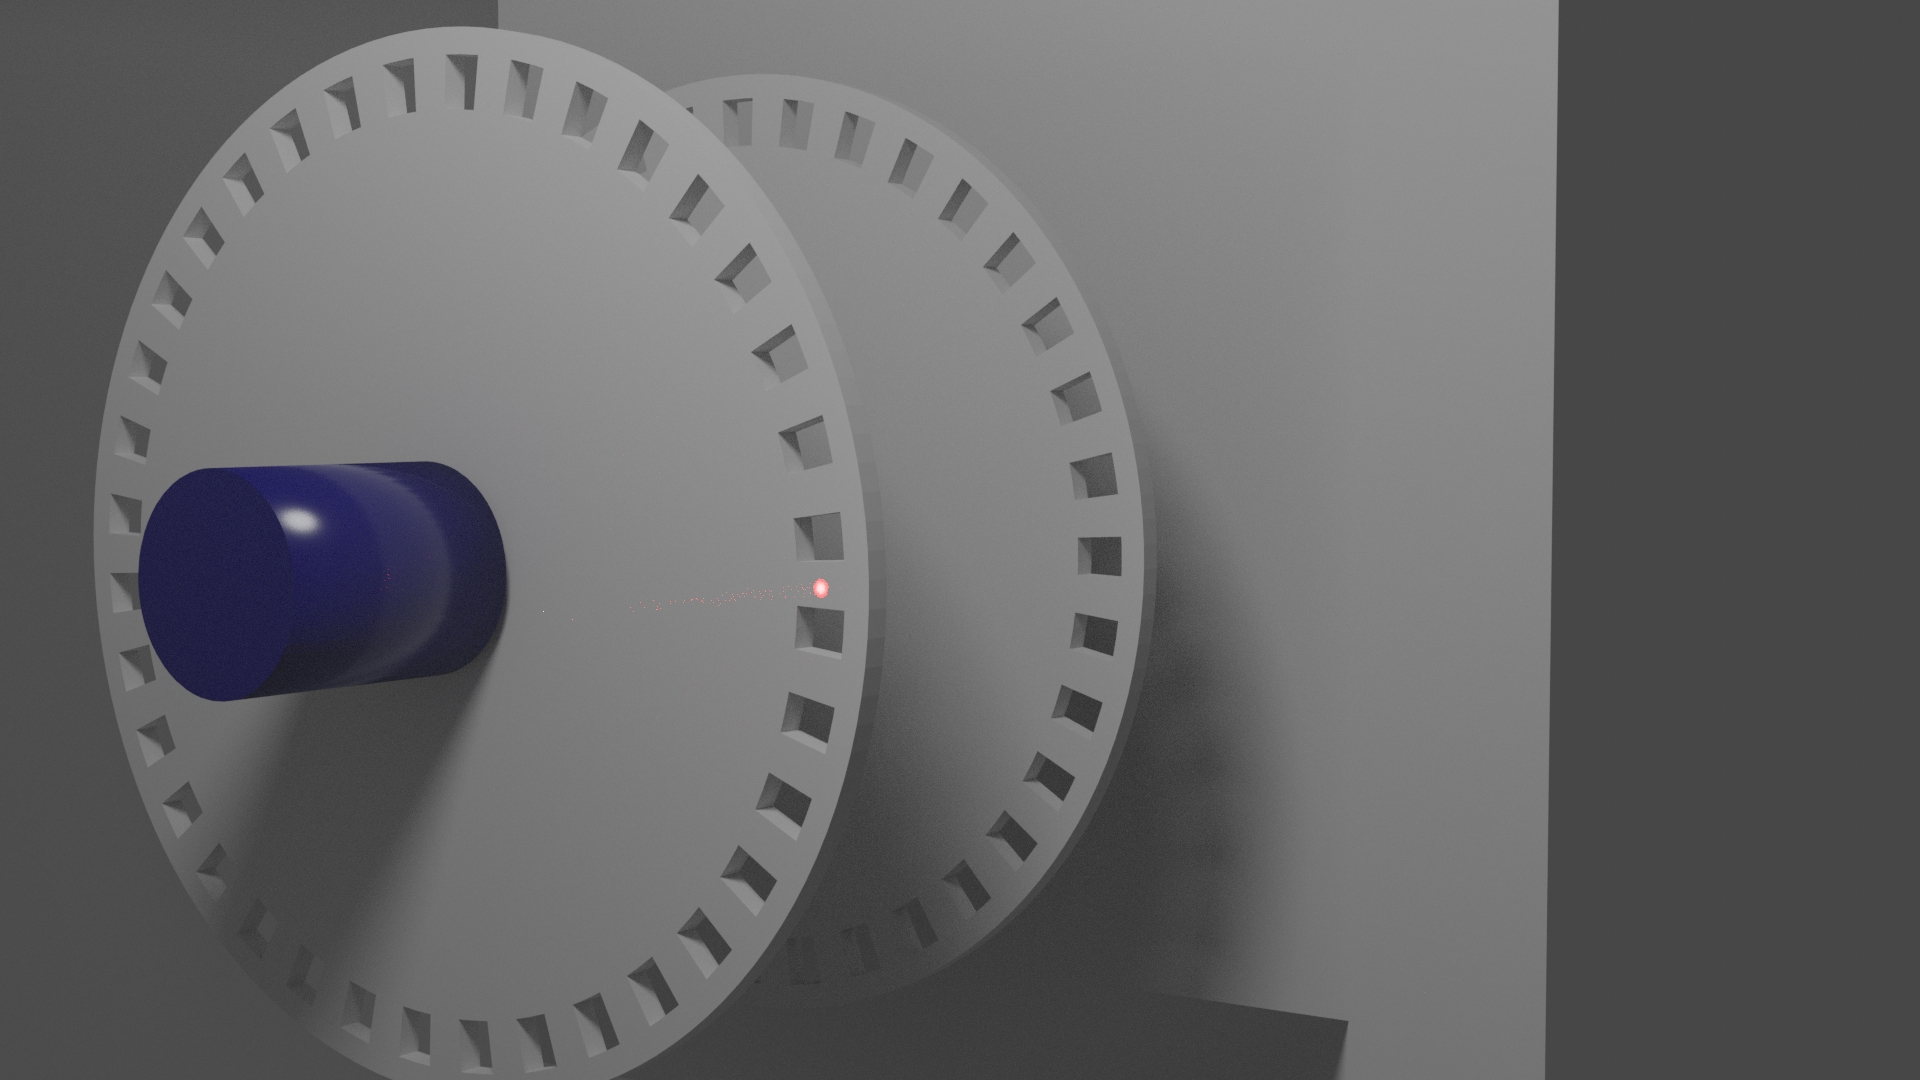
\includegraphics[width=\linewidth]{disc_3.png}
 \caption{Simulação do demonstrador - Posição 3}
 \label{fig:discs3}
\end{figure}


\subsection{Seguimento de um traçado com um braço robótico}\label{sec:robotic_arm}

% \subsubsection{O conceito}
A segunda proposta de solução para a dissertação em estudo trata-se do
controlo de um manipulador robótico do tipo 'braço' através da mesma
arquitetura de comunicação e de controlo descrita em \ref{sec:solution} e
\ref{sec:discs_project}. O objetivo deste braço robótico será fazer o
seguimento de um caminho, do estilo labirinto, com a sua ferramenta.
Esta poderá ser, por exemplo, um apontador laser (derivado do conceito
descrito em \ref{sec:discs_project}) ou, no caso de verificar viável, uma
massa de esparguete.

A utilização de um objeto tridimensional como ferramenta torna a ação de
percorrer um trajeto mais interessante e relevante para o objetivo.
Quando se considera a utilização de um apontador laser, este só tem
representação num plano bidimensional e portanto pode ser usada uma folha
de papel como suporte para o trajeto. Considerando a utilização de um
objeto tridimensional como ferramenta, como é o caso da massa de
esparguete, torna-se necessária a utilizaçao de um suporte tridimensional
com canais para definir o trajeto. No âmbito deste projeto, um suporte
em material como plástico PLA ou MDF é suficiente face às caraterísticas
de demonstrador didático.

\subsubsection{Manipulador do tipo braço robótico}
Um braço robótico é tipicamente composto por um conjunto de servo-motores,
onde cada um controla a posição de uma junta do manipulador e onde o
controlo simultâneo de todas as juntas permite controlar o manipulador
como um todo, podendo posicionar a ferramenta, que se encontra na extremidade,
numa posição pretendida. Esta posição é geralmente denominada de ponto
comandado (\emph{setpoint}).

O processo de cálculos matemáticos necessários à determinação da posição
de cada junta, com o objetivo de posicionar a ferramenta num dado ponto
do espaço é denominado cinemática inversa  (\emph{inverse kinematics}).
A cinemática inversa é geralmente calculada no planeador de trajetória,
cuja função é controlar o modo como o movimento é executado. Existem vários
tipos de movimentos possíveis, mas todos eles podem ser decompostos em
combinações dos seguintes tipos de movimento:

\begin{itemize}
 \item movimento livre (também conhecido por movimento no espaço das
 juntas), onde cada junta é controlada de modo independente e é usada
 quando apenas a posição final é importante e a trajetória que a ferramenta
 irá percorrer até atingir o ponto comandado não é relevante. Este movimento
 é caraterizado por ser um movimento rápido, onde todas as juntas iniciam
 e terminam o seu movimento em simultâneo, sendo para isso ajustadas as
 respetivas velocidades;
 \item movimento linear, onde é feita uma interpolação linear entre o
 ponto de partida e o ponto comandado, de maneira a que a ferramenta do
 manipulador passe por todos os pontos colineares com a reta que liga
 o ponto de comando e o ponto de partida. Este tipo de movimento é utilizado
 quando, por algum motivo, se pretende que a ferramenta se mova numa linha
 reta entre o ponto de partida e o ponto comandado.
 \item movimento circular, onde é executada uma interpolação circular
 entre o ponto de partida e o ponto de comando, sendo necessário fornecer
 o raio da circunferência que se pretende percorrer ou, em alternativa,
 um ponto que deve ser atingido durante a trajetória, que permite calcular
 internamente o raio da circunferência.
\end{itemize}

Como conhecemos da geometria, qualquer forma geométrica pode ser representada
através da sua decomposição em pontos singulares. Analogamente, um movimento
curvilíneo pode ser decomposto numa sequência de pontos discretos.
Idealmente usar-se-ia um número infinito de pontos mas, devido a limitações
computacionais, é necessário limitar o número de pontos desta decomposição,
baixando a precisão do movimento. O objetivo principal do planeador de
trajetória é fazer a computação dos pontos de posicionamento intermédio
para que seja possível realizar cada um destes tipos de movimento.
Estes pontos de comando são enviados para os controladores de posição de
cada eixo, geralmente do tipo \emph{PID}, para que estes movam a respetiva junta
para a posição pretendida.

\subsubsection{Conclusão}
Neste tipo de movimentos é fundamental que o controlo das várias juntas
do braço seja preciso e feito de um modo síncrono. É exatamente neste
conceito que este projeto se baseia, demonstrando que é necessária uma
comunicação rápida, de baixa latência e com capacidade de sincronização
de relógios para permitir a implementação de uma arquitetura de controlo
distribuída, inter-ligada por uma rede de comunicação de tempo real.
